\pdfbookmark{Summary}{label:summary}
\section*{General Summary}
This document concludes the 12th HGSFP Winter School that took place at
the University Center in Obergurgl from 16th to 20th of January 2019. In
total, 48 graduate students from Heidelberg and 10 lecturers participated
in the five-day event. The aim of the Winter School was to give students
the opportunity to get insights into other research fields in
Heidelberg apart from their own field. In the course of this, one of the
focal points was the scientific exchange between the students
themselves and students and lecturers in a friendly atmosphere. To this
end, we organized a scientific programme consisting of 10 lectures given
by speakers from Heidelberg and other universities and two poster
sessions with elevator talks (see Appendix A).


\subsection*{Participant Selection}
As expected, we received more applications for the school than spots were available. We therefore had to select participants from the pool of applicants, which we wanted to perform as fair as possible. We felt it was important to be both transparent about and accountable for our selection. For this reason, we imposed a selection algorithm, laid open the complete procedure (with anonymized data)\footnote{https://github.com/matiscke/HGSFPschoolParticipantSelection}, and explain what decisions went into the selection. In the following, we give an overview on how we selected the participants for the HGSFP winter school 2019.

\subsubsection*{Asking The Right Questions}
Designing the application form was perhaps the most difficult task, and it is at this stage that conference organizers will already want to put serious thought into the goals of the workshop and the ideal mix of participants to achieve those goals. It should be obvious, but you will only be able to include categories in your selection that you actually ask for.

\subsubsection*{Pre-selection}
Excluding speakers, we have 52 spots for the meeting. Our participant selection proceeded in two parts. In the first part, we rejected candidates outright who were either (1) duplicate entries or (2) candidates who had informed us that they would not be able to come. Two spots were reserved for the HGSFP representatives. Finally, we pre-selected the organizing committee, who needs to be present at the school. Thus, a total of 8 participants (6 organizers, 2 representatives) were pre-selected. We then anonymized our applicant pool by replacing names and other identifying information with a unique identifier. 

\subsubsection*{Participant Selection}
For the remaining 52 - 8 = 44 slots, we used the software \texttt{entrofy} to optimize our participant set based on a set of well-defined criteria on which the organizers agreed. It's worth noting here that this discussion took place before performing the selection, which then depended entirely on the goals for the selection and was independent of the input data set. 

\subsubsection*{Target Distributions}
The targets define the fraction of participants in the final output set who share the same value of a property (e.g. 25\% of participants should be affiliated with the HGSFP branch "Fundamental Interactions and Cosmology"). The target fractions must sum up to be smaller or equal to 1.0 for each category. If the target fractions sum to a value smaller than one, the algorithm will try to fill up categories to at least the given fractions, and will ignore that category for the rest of the optimization procedure. The resulting mix of participants in the final set for this category will thus be a combination of the input fractions and the distribution in the input sample, conditioned on the constraints set by the remaining categories. Below, we will go through each category one by one and lay out our reasoning for the categories chosen. The justification for our choices is an abbreviated version of a longer discussion the organizing committee had before starting the selection procedure. We should note at this point that there is no "correct" way to choose target fractions; the target fractions must necessarily always be a function of the objectives and goals of the workshop, as defined by the organizers.

\subsubsection*{Selection Goals}
Broadly, the goals we defined for the HGSFP Winter School 2019 for participant selection are the following:
\begin{itemize}
	\item enable every HGSFP student to attend one winter school during their PhD:
	\begin{itemize}
		\item[$\Rightarrow$] strongly favor applicants that have not attended a HGSFP winter school before
		\item[$\Rightarrow$] favor applicants that are longer into their PhD (since the clock is ticking...)
	\end{itemize}
	\item Reflect the student numbers of the different HGSFP branches
	\item Increase the participation of underrepresented minorities (in our case this translates to an effort for gender equality)
\end{itemize}
~\\
\textbf{HGSFP branch}\\
For the branch attribute, we aim to reflect the distribution of the overall branch affiliation

~\\
\textbf{Previous Winter School Attendance}\\
Derived from our top requirement, the acceptance of applicants with previous attendance of a winter school should be an exception. We decided if we allow previous attendees at all based on the oversubscription of the school. The latter was not very high, we therefore decided to accept applicants with previous attendence only via the waiting list. We enforce this criterion further below and do not solve for this parameter.

~\\
\textbf{Gender Identity}\\
Any social engineering involving gender is necessarily subject to scrutiny. Our choices here reflect our beliefs about what we would like the Winter School to be: We recognize that underrepresented minorities are particularly underrepresented in physics, which is reflected in the number of non-male PhD students. We also recognize studies that show that diverse groups outperform groups lacking diversity among several axes. Representation is important: we believe that minority participants might feel more comfortable participating if they do not feel singled out based on their gender.

Realizing that an equal representation of genders cannot be realized given the input set, we choose to set a goal fraction of female participants slightly higher than the corresponding share in the HGSFP and allow a sufficient margin for the option "Don't identify with either".

~\\
\textbf{PhD Duration}\\
We aimed to give senior PhD students that have not participated in a Winter School before an advantage in the selection, since they have less or no opportunities to re-apply next year.

~\\
Aside from the organizers and representatives, the entire procedure was performed entirely without names and based only on the candidates' responses and the complex optimization of the participant selection with respect to our goals. After the selection, all applicants were informed about the outcome and applicants in the 'accepted' list were asked to confirm their attendance within a specified period. Not all participants accepted our invitation on the first round. Free spots were filled with applicants from the waiting list on a first-come, first-served basis with regard to our notification emails. 

~\\
More detailed information about our selection procedure and an interactive Jupyter notebook that includes the original code can be found on\\
https://github.com/matiscke/HGSFPschoolParticipantSelection.








\subsection*{Lectures}
The lecture topics covered the six largest branches of the HGSFP and were
arranged in sessions of three parallel lectures each. In this way the
students had the possibility to choose the three topics they were most
interested in, while leaving enough free time for social activities and
exchange. The great majority of students preferred this format over a
tighter schedule with less parallel sessions (see Appendix B1). When
organizing the lectures, our main consideration was to choose
speakers that are known to give good introductory courses. We tried to
keep the lectures rather informal such that students felt animated to
ask questions and discussion developed during the sessions. The response
of the students to this style of lectures was very good and they
appreciated the broad range of topics ranging from String theory to Glacier
physics (see Appendix B2).

\subsection*{Poster Sessions}
The participants had the chance to present their own work in poster
sessions that took place on two of the evenings. We decided to keep
the short elevator talk sessions, that had first been introduced in the
winter school 2017, in place. In this short round of talks each student
got the chance to introduce his poster in a one minute pitch talk.
Again, the general feedback to these elevator talks was very good.
Following the tradition of the winter school, all students and lecturer
had the chance to elect the winner of the winter school poster price by
anonymous vote. The name of the winner will be engraved into the \textit{HGSFP
Wanderpokal}.

\subsection*{Venue}
The conference took place at the University Center in Obergurgl. The
great advantage of this venue is that it offers a lot of space with
several lecture rooms while being in direct proximity to a ski resort.
This goes hand in hand with the spirit of the winter school of combining
a rich lecture programme with enough time for social activities as
skiing or hiking. The local staff was very helpful and contributed to
everything running smoothly during our stay. The venue got an excellent
rating by all participants and both the very good food and very clean
rooms where highly appreciated. Even though the University Center
significantly increased its prises over the years, we believe that it is
still completely out of competition for what it offers.


\subsection*{Travel}
After the evaluation of the winter school 2017, we had decided to travel
by bus over night again. Even though travelling over night is
certainly quite exhausting, the great majority of students had preferred
this option over losing the additional time by travelling during the
day. This years survey shows a very similar outcome.

\subsection*{Social Event}
Following the tradition, the first evening of the Winter School was
devoted to the social event — Eisstockschiessen. The participants
appreciated this chance to get to know each other very
much and, to our delight, most of the speakers joined as well. As our
survey shows, some of the students did even wish for an additional
organized social event on the last evening.

\subsection*{Final Remarks}
Summarized, we think that this years Winter School was a great success.
The feedback of students and lectures was very good and we believe that
the goals of the school could be achieved. Everything went exactly as
planned and the five days passed without any problems arising. We are
very thankful for the great organizational and financial support of the
HGSFP for this event and we hope that the tradition of the Winter School
will be carried on in the future.


\newpage
\section*{A $\qquad$ Schedule of the HGSFP Winterschool 2018}

\pdfbookmark{A Schedule}{label:appa}
\begin{figure}[h!]
\centering
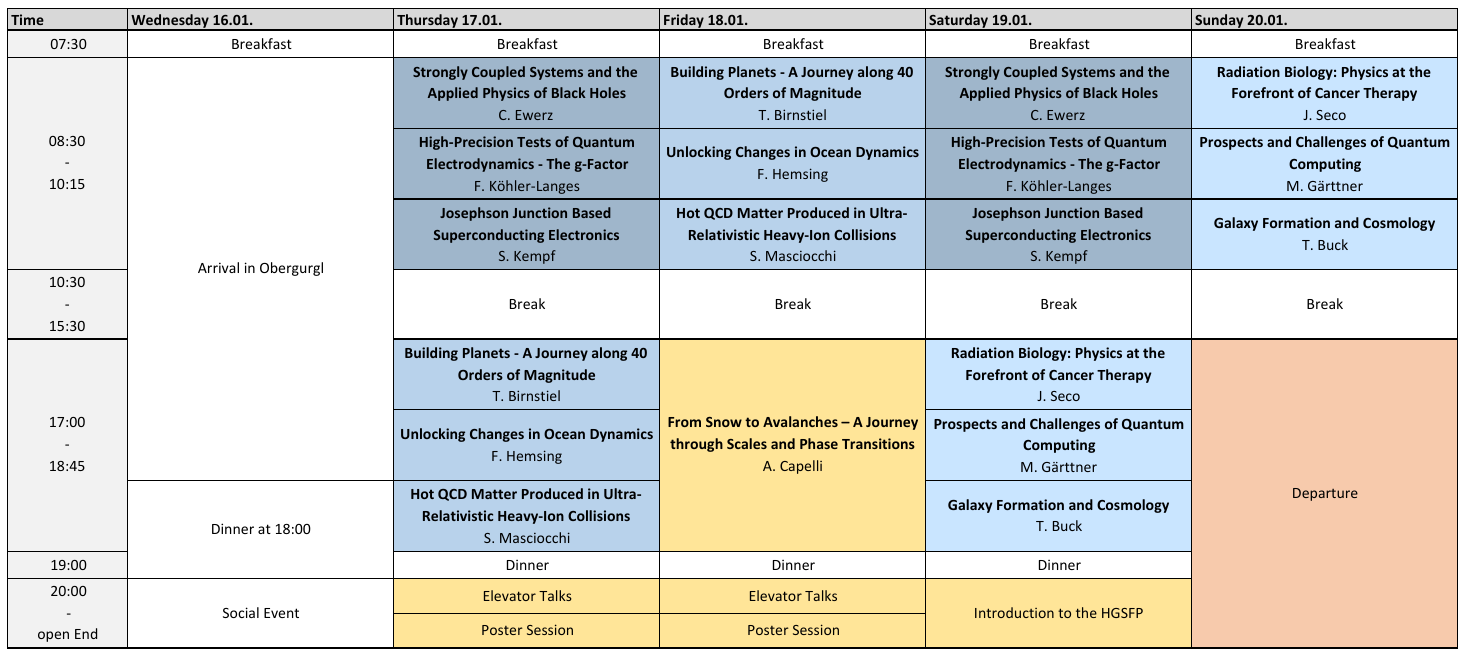
\includegraphics[scale=0.66, angle = 90 ]{figures/Program.jpg}
\end{figure}


\section*{B $\qquad$ Evaluation}

\newpage